\documentclass[letterpaper, 11pt]{article}

% set version variable
\newcommand{\versionnumber}{0.1}

% russian language
\usepackage[utf8]{inputenc}
\usepackage[T2A]{fontenc}
\usepackage[english, russian]{babel}
\usepackage{algorithmicx}
\usepackage{algpseudocode}
\usepackage{graphicx}
\usepackage{caption}
\usepackage{subcaption}
\usepackage{amsmath}


% math
\usepackage{amsmath}

\usepackage{amssymb} % some math symbols


% enumerate
\usepackage{enumerate}

% set type and margins of the page
\usepackage{geometry}  % document margins
\geometry{letterpaper, left=1.4in, right = 1.4in, top = 1.7in, bottom = 1.7in}

% color links in content
\usepackage{hyperref}
\hypersetup{
    colorlinks=true,
    linkcolor=red,
    urlcolor=blue,
    linktoc=all
}

% indent at first \par after section
\usepackage{indentfirst}

% fixed table and figures in section
\usepackage{float}

% colors
\usepackage{color}
\usepackage[usenames,dvipsnames]{xcolor}

\newcommand{\prob}{\mathrm{P}}
\newcommand{\expe}{\mathrm{E}}
\newcommand{\var}{\mathrm{D}}
\newcommand{\tr}{\mathrm{tr}}
\newcommand{\KK}{\mathbf{K}}
\newcommand{\XX}{\mathbf{X}}
\newcommand{\MM}{\mathbf{M}}
\newcommand{\Cov}{\mathrm{Cov}}
\newcommand{\Var}{\mathrm{Var}}

% paragraph indent
\setlength{\parskip}{0.5em}

\title{\large{Краткий конспект}\\
\LARGE{Лекция 3. Локальное выравнивание. Алгоритм Смита-Ватермана. BLAST}\\
\normalsize{\textcolor{NavyBlue}{draft version}}}
\date{7 марта, 2016}
\author{Д. Ищенко\thanks{МФТИ} \and \underline{Б. Коварский\footnotemark[1]}
\and И. Алтухов\footnotemark[1] \and Д. Алексеев\footnotemark[1]}

\begin{document}
\maketitle
\thispagestyle{empty}
\clearpage

% let's go
\section{Матрицы замен и аффинные штрафы}

На прошлой лекции, используя подход динамического программирования, мы с вами построили алгоритм для поиска пути в редакционном графе, минимизирующего редакционное расстояние среди всевозможных выравниваний, используя рекуррентное соотношение:

$$d_{i,j}=
\min
\begin{pmatrix}
	d_{i-1,j}+1, \\
	d_{i,j-1}+1, \\
	d_{i-1,j-1}+[v_i\ne w_j]
\end{pmatrix}$$

Где, $d_{i,j}=d_L(V^i,W^j)$ расстояние Левенштейна между префиксами длины $i$ и $j$ строк $V$ и $W$ соответственно

В биологических приложениях обычно вместо задачи минимизации редакционного расстояния обычно решают задачу максимизации сходства. За совпадение награждают, а за несовпадения и разрывы (вставки-удаления) штрафуют.

Рекуррентное соотношение нужно переписать:

$$s_{ij}=
\max
\begin{pmatrix}
	s_{i-1,j}-1, \\
	s_{i,j-1}-1, \\
	s_{i-1,j-1}-[v_i\ne w_j]+[v_i = w_j]
\end{pmatrix}$$

Штраф здесь фиксирован: мы всегда штрафуем на единицу за несовпадение и разрыв, и прибавляем единицу в случае совпадения. Для того чтобы перейти от выравнивания абстрактных строк к биологически осмысленному выравниванию этого недостаточно. Нам нужно решить две задачи, во-первых, принять во внимание тип замены, какая аминокислота/нуклеотид на какую/какой меняется, а во-вторых, размер индела.

Первая задача легко решается, мы вводим \textit{матрицу замен} (substitution matrix) - симметричную матрицу в которой храним для каждой пары символов штраф, для случая, когда один символ из пары меняется на другой символ из пары. При этом $\delta(a,a)\ge 0$. Если в матрицу замен в качестве символа внести еще и символ разрыва '-', рекуррентное соотношение приобретает совсем простой вид:

$$s_{ij}=
\max
\begin{pmatrix}
	s_{i-1,j}+\delta(v_i,-), \\
	s_{i,j-1}+\delta(-,w_i), \\
	s_{i-1,j-1}+\delta(v_i,w_j),
\end{pmatrix}$$

\begin{figure}
\centering
\begin{subfigure}{.6\textwidth}
  \centering
  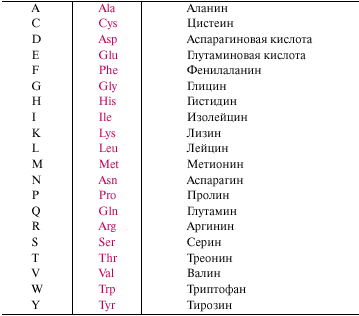
\includegraphics[width=\linewidth]{images/iupac_codes.png}
  \caption{}
  \label{fig:sub1}
\end{subfigure}%
\begin{subfigure}{.6\textwidth}
  \centering
  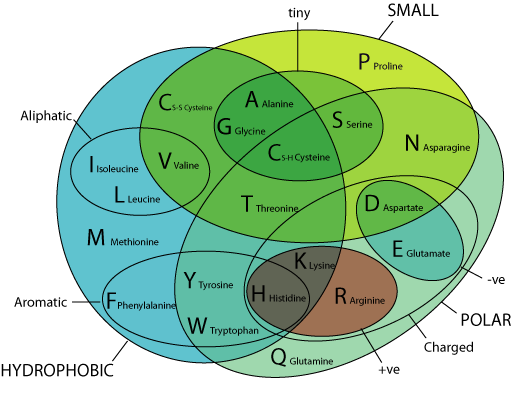
\includegraphics[width=\linewidth]{images/aa_properties.png}
  \caption{}
  \label{fig:sub2}
\end{subfigure}
\begin{subfigure}{.9\textwidth}
  \centering
  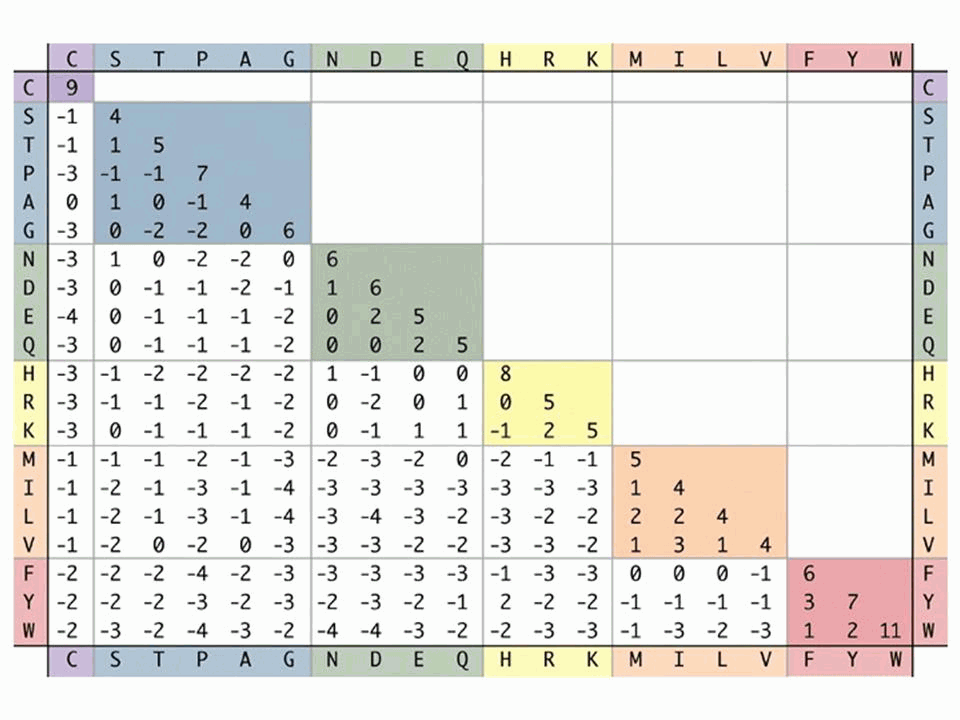
\includegraphics[width=1.2\linewidth]{images/BLOSUM.png}
  \caption{}
  \label{fig:sub2}
\end{subfigure}
\caption{(a)Однобуквенные и трехбуквенные коды IUPAC, кодирующие аминокислоты; (b) Диаграмма сходства аминокислот по физико-химическим свойствам; (c)-матрица BLOSUM}
\label{fig:test}
\end{figure}

Наиболее часто в молекулярной биологии используются матрицы замен BLOSUM62 и PAM250.

Веса в этих матрицах замен извлекаются из статистики выравнивания родственных белков. Исторически первая (Margaret Dayhoff, 1978) матрица замен PAM  (point accepted mutation - закрепившаяся точечная мутация) конструировалась по глобальным выравниваниям белков со сходством не менее 85\%.

Использованный Дэйхофф методологический подход сравнения близкородственных последовательностей не всегда оптимален при анализе последовательностей, связанных дальним родством. Эта проблема решается в матрицах класса BLOSUM (Block substitution matrices - матрица замен в блоках, Henikoff and Henikoff, 1992). Матрицу BLOSUM62 (BLOcks SUbstitution Matrix - матрица замен в блоках).

Для построения матрицы BLOSUM строились не глобальные, а локальные выравнивания и анализировались частоты замен аминокислот в высококонсервативных регионах аминокислотных последовательностей, имеющих не менее чем 62\% сходство (отсюда цифра 62 в названии). Высококонсервативным регионам в выравниваниях соответствуют блоки без разрывов (без инделов - отсюда BLOcks в названии). Что такое локальное выравнивание и в чем его отличие от глобального, обсудим далее по лекции.

В качестве значения штрафов в этой матрице используется \textit{логарифм отношения шансов} (log odd ratio) - величина, показывающая насколько вероятность наблюдаемая частота аминокислотной замены выше ожидаемой:
$$\delta_{ij}=A\log{\frac{p_{ij}}{q_i q_j}} \sim \log \frac{\prob (Observed)}{\prob (Expected)}$$

$p_{ij}$ - наблюдаемая частота встречаемости аминокислот $i$ и $j$  в паре среди всевозможных выравниваний. Фактически, это вероятность замены аминокислоты $i$ на аминокислоту $j$

$q_i$ - частота встречаемости $i$-й аминокислоты в анализируемых последовательностях.

$q_i*q_j$ - ожидаемая частота встречаемости пар аминокислот $i$ и $j$  в паре среди всех выравниваний. Т.е. вероятность, что две аминокислоты окажутся в паре, если бы случайным образом записали одну последовательность под другой.

$A$ - нормировочный множитель, для того чтобы значения штрафов были близки к небольшим целым числам.

Можно заметить, что матрица BLOSUM имеет блочное устройство: пары аминокислот со схожими физико-химическими свойствами имеют в матрице BLOSUM положительные значения отношения шансов. Чем сильнее отличия аминокислот, тем более серьезный эффект будут иметь замены и тем реже такой тип замен встречается и тем меньше будет отношения шансов (больше штраф).

Далее нам хотелось бы, чтобы штраф за индел как-то зависел от его размера. Эта задача проистекает из наблюдения, что каждый индел, вне зависимости от его размера - это чаще всего одно эволюционное событие. Поэтому выравнивание с небольшим числом крупных инделов предпочтительнее выравнивания со множеством мелких инделов. Данная задача решается введением \textit{аффинного штрафа} за разрыв (affine gap penalty): $$\sigma(l)=\sigma_0+\epsilon l$$
Где $\sigma_0$ - штраф за инициирование разрыва, $\epsilon$ - штраф за увеличение разрыва на единицу.

Использование аффинного штрафа требует небольшой модификации алгоритма, но мы не будем останавливаться на этом.

\section{Локальное выравнивание}

Давайте еще раз обсудим, для чего нужно глобальное выравнивание. Итак, глобальное выравнивание нужно когда мы хотим обнаружить изменения, накопленные в ходе эволюции между двумя родственными последовательностями, в общем и целом не сильно утратившими сходство, например, между последовательностями белков, входящих в одно семейство
.
Но зачастую белки содержат множество структурно и функционально независимых единиц или \textit{доменов}. Как и гены, домены образуют семейства. Эволюционно родственные семейства доменов в свою очередь объединяются в \textit{кланы}. Из-за происходившей в ходе эволюции рекомбинации генов разные домены развивались независимо и у неродственных генов некоторые домены или мотивы могут оказаться схожими. Информацию по известным на сегодняшний день семействам доменов можно найти на странице базы данных Pfam (\url{http://pfam.xfam.org/}). К примеру, \href{http://pfam.xfam.org/family/browse?browse=top%20twenty}{двадцать самых распространенных доменов}.

В качестве примера доменной организации, можно привести гомеозисные, HOX-гены, определяющие процессы роста и дифференцировки в организме. Гомеозисные гены кодируют транскрипционные факторы, определяя тип развития ткани и органа. Гомеозисные гены содержат гомеобокс — последовательность из 180 пар нуклеотидов ДНК. Ошибки экспрессии гомеозисных генов приводят к крупным изменениям в морфологии животного. Поэтому область гомеобокса крайне консервативна, хотя другие области гомеозисных генов могут дивергировать очень сильно, а так же иметь свой уникальный набор доменов (на \href{http://pfam.xfam.org/family/PF05920#tabview=tab1}{странице} приведены гены с наличием HOX-домена).

Для поиска небольших гомологичных фрагментов в сильно отличающихся последовательностях глобальное выравнивание непригодно. Для этого используется \textit{локальное выравнивание}. Для чего нужно локальное выравнивание? Локальное выравнивание нужно, когда мы хотим определить \textit{схожие фрагменты в отличающихся последовательностях}. А глобальное, как мы помним, нужно, когда мы хотим определить \textit{отличия в схожих последовательностях}. Важно это различать.

\begin{figure}
  \centering
  % Requires \usepackage{graphicx}
  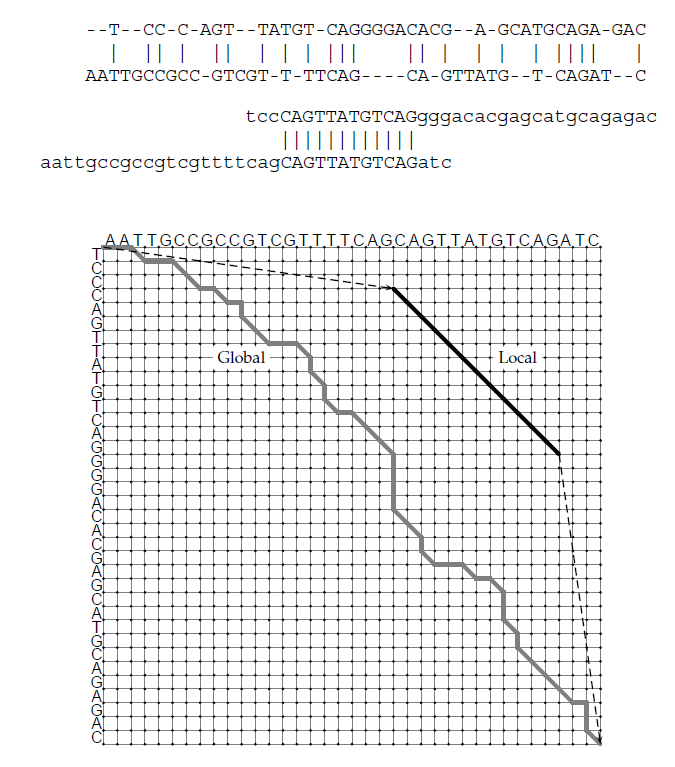
\includegraphics[width=0.7\linewidth]{images/local_and_global.png}\\
  \caption{Глобальное и локальное выравнивание двух нуклеотидных последовательностей с консервативным участком и пути в редакционном графе, соответствующие этим выравниваниям (схема взята из [3])}\label{fig:second}
\end{figure}


Задачу локального выравнивания формально можно определить так. Для двух строк $V^n$ и $W^m$, среди всевозможных глобальных выравниваний всех подстрок найти пару подстрок с наибольшей величиной сходства (similarity score) глобального выравнивания. В терминах редакционного графа это означает следующее. В глобальном выравнивании среди путей из истока $(0,0)$ в сток $(n,m)$ мы ищем путь c наибольшим весом. В локальном выравнивании же ищем путь из произвольного истока $(i_1,j_1)$ в произвольный сток $(i_2,j_2)\quad i_1\le i_2, j_1\le j_2$, обладающий наибольшим весом среди всех путей в графе.

Проблема перебора всех стоков и истоков решается на удивление изящно. В 1981 Темпл Смит и Майкл Ватерман показали, что задача локального выравнивания может быть сведена к поиску пути c наибольшим весом из истока $(0,0)$ в произвольный сток $(i,j)$ в модифицированном редакционном графе, в котором добавлены ребра с нулевым весом из $(0,0)$ во все остальные вершины.

\begin{figure}
  \centering
  % Requires \usepackage{graphicx}
  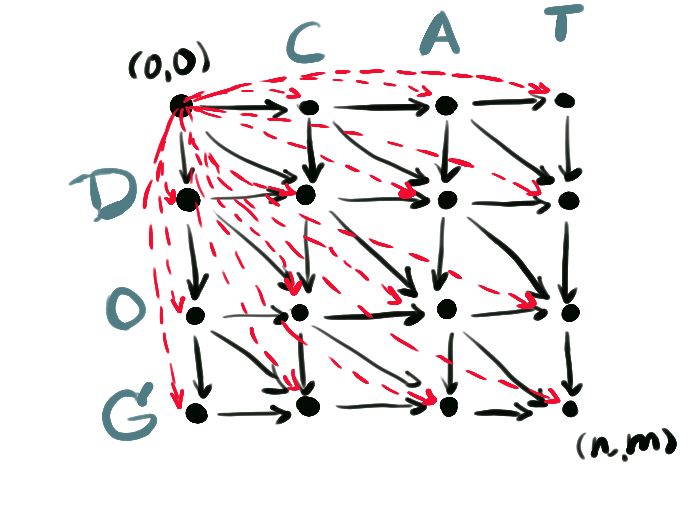
\includegraphics[width=0.7\linewidth]{images/edit_graph_modified.png}\\
  \caption{Модифицированный редакционный граф с ребрами нулевого веса, соединяющие исток и все остальные вершины}\label{fig:third}
\end{figure}

Для решения этой задачи необходимо переписать рекуррентное соотношение следующим образом:

$$s_{ij}=
\max
\begin{pmatrix}
	0, \\
	s_{i-1,j}+\delta(v_i,-), \\
	s_{i,j-1}+\delta(-,w_i), \\
	s_{i-1,j-1}+\delta(v_i,w_j),
\end{pmatrix}$$

Заметим, что при таком рекуррентном соотношении, матрица весов выравниваний будет заполнена неотрицательными значениями: $s_{i,j}>0$, значит суммарный вес любого пути в редакционном графе также неотрицательный, как только вес становится меньше нуля по любому из направлений он обнуляется.

При помощи рекуррентного соотношения мы заполняем таблицу c весами $s_{ij}$. После чего находим $\arg\max_{i,j}s_{ij}$ и, двигаясь из стока по указателям, восстанавливаем оптимальное локальное выравнивание:


\begin{algorithmic}[2]
\Procedure{SWLocalAlignment}{$V,W$}
\State $S\gets [\quad]$
\State $B\gets [\quad]$\Comment{Создаем массив для хранения направлений}
\For{$i\gets 0, n$}
\State $S[i,0]\gets 0$
\State $B[i,0]\gets "*"$\Comment{* - условный символ для позиций с нулевым весом}
\EndFor

\For{$j\gets 0, m$}
\State $S[0,j]\gets 0$
\State $B[0,j]\gets "*"$
\EndFor

\For{$i\gets 1, n$}
\For{$j\gets 1, m$}

\State $S[i,j]\gets 0$
\State $B[i,j]\gets "*"$

\If{$S[i,j] < S[i-1,j-1]+\delta(V[i],W[j])$}
\State $S[i,j]\gets S[i-1,j-1]+\delta(V[i],W[j])$
\State $B[i,j]\gets "\searrow"$
\EndIf

\If{$S[i,j] < S[i-1,j]+\delta(V[i],-)$}
\State $S[i,j] \gets S[i-1,j-1]+\delta(V[i],-)$
\State $B[i,j]\gets "\rightarrow"$
\EndIf

\If{$S[i,j] < S[i,j-1]+\delta(-,W[j])$}
\State $S[i,j] \gets S[i,j-1]+\delta(-,W[j])$
\State $B[i,j]\gets "\downarrow"$
\EndIf

\EndFor
\EndFor
\State \textbf{return} $B$
\EndProcedure
\end{algorithmic}


\section{BLAST}

Мы с вами обсудили два базовых агоритма для построения глобального и локального выравнивания - алгоритм Нидлмана-Вунша и Смита-Ватермана. Оба алгоритма - не модельные примеры, не дань истории, а вполне себе рабочие алгоритмы, использующиеся сегодня, когда требуется высокое качество выравнивания. Оба алгоритма доступны онлайн, например, на сайте Европейского Биоинформатического института: \href{http://www.ebi.ac.uk/Tools/psa/emboss_needle/}{EMBOSS Needle}, \href{http://www.ebi.ac.uk/Tools/psa/emboss_water/}{EMBOSS Water}.

Сложность алгоритма Смита-Ватермана, как и алгоритма Нидлмана-Вунша $O(nm)$ по времени и по памяти. Можно ли улучшить эти оценки? Оказывается, используя подход "разделяй и властвуй" (divide and conquer) мы можем уменьшить требования по памяти. У алгоритма Хиршберга, реализующего такой подход, сложность по памяти $O(\min (n,m))$. Временную оценку без падения точности улучшить нельзя.

Скорость особенно критична, во-первых, когда мы одновременно выравниваем более двух последовательностей, выполняем так называемое множественное выравнивание. Сложность алгоритмов Смита-Ватермана и Нидлмана-Вунша растет полиномиально с количеством последовательностей, т.е. для одновременного выравнивания 10 последовательностей она будет равна $O(n^{10})$.

Во-вторых, рассмотренные алгоритмы непригодны, если мы выравниваем одну последовательность на большой набор последовательностей. В этом случае сложность $O(kn^2)$, где $k$ - количество последовательностей в базе данных. В базе данных NCBI RefSeq(\url{http://www.ncbi.nlm.nih.gov/refseq/}) на 20 января 2016 хранится 58.5 млн. белковых последовательностей для 58 тыс. организмов. Медианное значение длины гена $300$ аминокислот. Если мы захотим сравнить неизвестную последовательность с последовательностями в RefSeq нам понадобится выполнить 5 трлн. операций. 100 млн. операций на домашнем компьютере - это примерно одна секунда вычислений. Значит, чтобы выполнить нужные вычислений для одной последовательности необходимо 50 000 секунд, порядка тринадцати часов.

Что делать? Использовать различные эвристики, и ценою снижения точности увеличить скорость работы. Один такой эвристический алгоритм столь часто используется любым биологом, что мимо пройти было моветоном. Речь идет об алгоритме BLAST (Basic Local Alignment Search Tool). BLAST доступен онлайн по адресу: \url{http://blast.ncbi.nlm.nih.gov/Blast.cgi}

BLAST нужен когда у вас есть неизвестная последовательность и вы хотите найти все известные последовательности хоть как-то похожие на нее. Рассмотрим следующий пример. В 1990 году была опубликована книга Майкла Крайтона "Парк Юрского Периода", по которой впоследствии сняли фильм. На одной из страниц приведен якобы фрагмент генома динозвра в 1200 нуклеотидов:

\begin{verbatim}
>JurassicPark DinoDNA from the book Jurassic Park
gcgttgctgg cgtttttcca taggctccgc ccccctgacg agcatcacaa aaatcgacgc
ggtggcgaaa cccgacagga ctataaagat accaggcgtt tccccctgga agctccctcg
tgttccgacc ctgccgctta ccggatacct gtccgccttt ctcccttcgg gaagcgtggc
tgctcacgct gtaggtatct cagttcggtg taggtcgttc gctccaagct gggctgtgtg
ccgttcagcc cgaccgctgc gccttatccg gtaactatcg tcttgagtcc aacccggtaa
agtaggacag gtgccggcag cgctctgggt cattttcggc gaggaccgct ttcgctggag
atcggcctgt cgcttgcggt attcggaatc ttgcacgccc tcgctcaagc cttcgtcact
ccaaacgttt cggcgagaag caggccatta tcgccggcat ggcggccgac gcgctgggct
ggcgttcgcg acgcgaggct ggatggcctt ccccattatg attcttctcg cttccggcgg
cccgcgttgc aggccatgct gtccaggcag gtagatgacg accatcaggg acagcttcaa
cggctcttac cagcctaact tcgatcactg gaccgctgat cgtcacggcg atttatgccg
caagtcagag gtggcgaaac ccgacaagga ctataaagat accaggcgtt tcccctggaa
gcgctctcct gttccgaccc tgccgcttac cggatacctg tccgcctttc tcccttcggg
ctttctcatt gctcacgctg taggtatctc agttcggtgt aggtcgttcg ctccaagctg
acgaaccccc cgttcagccc gaccgctgcg ccttatccgg taactatcgt cttgagtcca
acacgactta acgggttggc atggattgta ggcgccgccc tataccttgt ctgcctcccc
gcggtgcatg gagccgggcc acctcgacct gaatggaagc cggcggcacc tcgctaacgg
ccaagaattg gagccaatca attcttgcgg agaactgtga atgcgcaaac caacccttgg
ccatcgcgtc cgccatctcc agcagccgca cgcggcgcat ctcgggcagc gttgggtcct
gcgcatgatc gtgctagcct gtcgttgagg acccggctag gctggcgggg ttgccttact
atgaatcacc gatacgcgag cgaacgtgaa gcgactgctg ctgcaaaacg tctgcgacct
atgaatggtc ttcggtttcc gtgtttcgta aagtctggaa acgcggaagt cagcgccctg
\end{verbatim}

Что значит эта последовательность? В начале 90-х базы данных последовательностей были еще крайне скудны, тем не менее молекулярный биолог Марк Богуски не поленился "забластовать" этот кусок (\href{http://markboguski.net/docs/publications/BioTechniques-1992.pdf}{статья} Богуски). Как вы, наверное, догадываетесь, к геному динозавра этот фрагмент не имеет отношения. А к чему имеет, \href{http://blast.ncbi.nlm.nih.gov/Blast.cgi?PROGRAM=blastn&PAGE_TYPE=BlastSearch&LINK_LOC=blasthome}{попробуйте выяснить самостоятельно}.

На этом история с "Парком Юрского" не заканчивается. В 1995 Крайтон выпустил продолжение книги, пригласив Богуски как консультанта. В книге снова приводился новый фрагмент генома динозавра. Что-то похожее у динозавра могло действительно быть :-).

\begin{verbatim}
>LostWorld DinoDNA from the book The Lost World
gaattccgga agcgagcaag agataagtcc tggcatcaga tacagttgga gataaggacg
gacgtgtggc agctcccgca gaggattcac tggaagtgca ttacctatcc catgggagcc
atggagttcg tggcgctggg ggggccggat gcgggctccc ccactccgtt ccctgatgaa
gccggagcct tcctggggct gggggggggc gagaggacgg aggcgggggg gctgctggcc
tcctaccccc cctcaggccg cgtgtccctg gtgccgtggg cagacacggg tactttgggg
accccccagt gggtgccgcc cgccacccaa atggagcccc cccactacct ggagctgctg
caaccccccc ggggcagccc cccccatccc tcctccgggc ccctactgcc actcagcagc
gggcccccac cctgcgaggc ccgtgagtgc gtcatggcca ggaagaactg cggagcgacg
gcaacgccgc tgtggcgccg ggacggcacc gggcattacc tgtgcaactg ggcctcagcc
tgcgggctct accaccgcct caacggccag aaccgcccgc tcatccgccc caaaaagcgc
ctgcgggtga gtaagcgcgc aggcacagtg tgcagccacg agcgtgaaaa ctgccagaca
tccaccacca ctctgtggcg tcgcagcccc atgggggacc ccgtctgcaa caacattcac
gcctgcggcc tctactacaa actgcaccaa gtgaaccgcc ccctcacgat gcgcaaagac
ggaatccaaa cccgaaaccg caaagtttcc tccaagggta aaaagcggcg ccccccgggg
gggggaaacc cctccgccac cgcgggaggg ggcgctccta tggggggagg gggggacccc
tctatgcccc ccccgccgcc ccccccggcc gccgcccccc ctcaaagcga cgctctgtac
gctctcggcc ccgtggtcct ttcgggccat tttctgccct ttggaaactc cggagggttt
tttggggggg gggcgggggg ttacacggcc cccccggggc tgagcccgca gatttaaata
ataactctga cgtgggcaag tgggccttgc tgagaagaca gtgtaacata ataatttgca
cctcggcaat tgcagagggt cgatctccac tttggacaca acagggctac tcggtaggac
cagataagca ctttgctccc tggactgaaa aagaaaggat ttatctgttt gcttcttgct
gacaaatccc tgtgaaaggt aaaagtcgga cacagcaatc gattatttct cgcctgtgtg
aaattactgt gaatattgta aatatatata tatatatata tatatctgta tagaacagcc
tcggaggcgg catggaccca gcgtagatca tgctggattt gtactgccgg aattc
\end{verbatim}


Так как работает BLAST? Ключевая идея BLAST проистекает из наблюдения, что если локальное выравнивание осмысленно, в нем будут встречаться участки, обладающих высоким сходством - high-score segment pairs. Если их совсем нет, то последовательности не обладают каким-либо сходством и выравнивать их и не нужно. То есть еще до выполнения выравнивания мы можем отбросить последовательности лишенные сходства с заданной, если в них отсутствуют сегменты сходства минимально возможной длины.

Для этого заданная последовательность разбивается на слова - всевозможные подстроки наперед заданного размера, так называемые k-меры. Для аминокислотных последовательностей стандартный размер слова - 6, нуклеотидных - 11. Размер слова $k$ - это первый параметр алгоритма.

Затем к полученным словам добавляются "соседние" слова. Т.е. k-меры обладающие достаточным сходством с исходными. Минимальный порог сходства $T$ - второй параметр алгоритма.

После того как, мы определили все необходимые слова, мы ищем в базе данных строки, в которых встречается хотя бы одно из слов. Так как строки в базе данных можно предобработать, то поиска интересующего слова в строке занимает константное время, всю строку просматривать не приходится. Если в некоторой строке мы нашли слово, мы пытаемся продлить слово влево и вправо, т.е. строим выравнивание вправо и влево, пока сходство между двумя выравненными последовательностями не станет меньше $T$.

\begin{figure}
  \centering
  % Requires \usepackage{graphicx}
  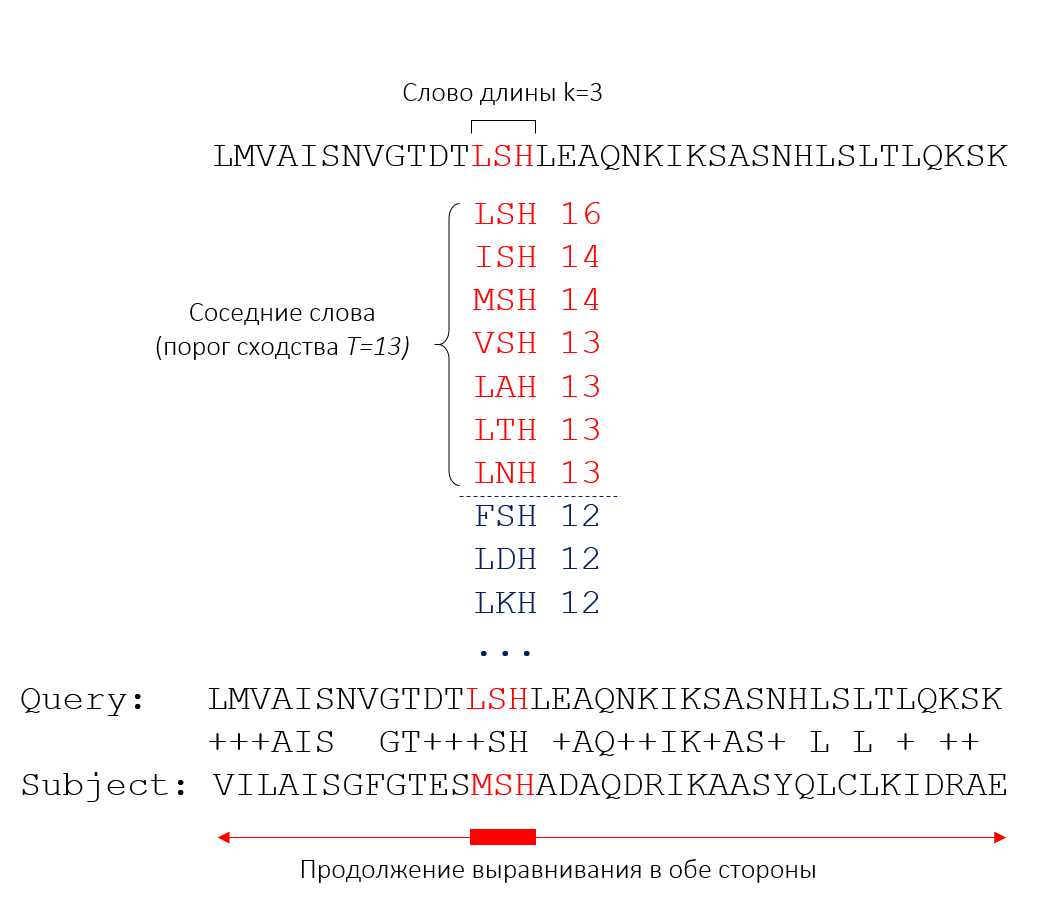
\includegraphics[width=0.9\linewidth]{images/blast_scheme.png}\\
  \caption{Схема работы алгоритма BLAST для поиска HSP: разбиение искомой (query) последовательности на слова $\rightarrow$ определение соседних слов  $\rightarrow$ поиск слов среди последовательностей в базе  $\rightarrow$ продление выравнивания в обе стороны}\label{fig:third}
\end{figure}

Второй важный компонент алгоритма состоит в определении достоверности найденных таким образом HSP. Почему важный? В случае выравнивания небольшого числа последовательностей мы таким вопросом не озадачиваемся. Но когда счет последовательностей идет на миллионы, даже если вероятность случайного совпадения  между двумя последовательностями мала, число совпадений может быть ненулевым.

Статзначимость найденных HSP оценивается посредством e-value. E-value - ожидаемое количество выравниваний с весом (score) $S$ больше заданного. Чем меньше e-value тем надежнее результат поиска, тем меньше вероятность, что совпадение случайно. E-value для последовательностей длины $n$ и $m$ рассчитывается как:

$$E(S)=Kmn \exp(-\lambda S)$$

Количество последовательностей $k$ со скором больше заданного будет распределено по Пуассону:

$$\prob(k)=\frac{E^k}{k!}e^{-E}$$

Тогда вероятность того, что для случайных выравниваний будет найдено как минимум одно со скором больше заданного равна:

$$P=1-\prob(k=0)=1-e^{-E}$$

Данная величина носит название p-value выравнивания. Параметры $K$ и $\lambda$, фигурирующие в $E(S)$ зависят от количества последовательностей в базе поиска и еще ряда настроек. Подробнее о их определении можно прочитать в \href{http://www.ncbi.nlm.nih.gov/pmc/articles/PMC53667/pdf/pnas01031-0226.pdf}{статье}.

%Статистика BLAST строится на распределении Гумбеля. Распределение Гумбеля - распределение с плотностью
%$f(x)=\frac{1}{\beta}\exp{(\frac{x-\alpha}{\beta}-\exp{(\frac{x-\alpha}{\beta})})}$ и функцией распределения:
%$F(x)=1-\exp(-\exp(\frac{x-\alpha}{\beta}))$

%Распределение Гумбеля возникает как распределение веса локального выравнивания между двумя случайными строками. Вероятность, что две случайные строки будут иметь вес выравнивания $S\ge x$ равно:

%$$p=\prob(S\ge x)=F(x)$$

\section{Ссылки}
\begingroup
\renewcommand{\section}[2]{}%
\begin{thebibliography}{7}
\bibitem{Frank}
Gusfield D. Algorithms on strings, trees and sequences: computer science and computational biology. – Cambridge university press, 1997.
\bibitem{Frank}
Дасгупта С., Пападимитриу Х., Вазирани У. Алгоритмы – Издательство МЦНМО, 2014.
\bibitem{Frank}
Jones N., Pevzner P. An Introduction to Bioinformatics Algorithms – MIT Press, 2004.
\end{thebibliography}


\end{document} 
